\documentclass[11pt,letterpaper,boxed]{hmcpset}
\usepackage{fullpage}
\setlength{\parskip}{6pt}
\setlength{\parindent}{0pt}
\usepackage[margin=1in]{geometry}
\usepackage{graphicx}
\usepackage{enumerate}
\usepackage{marvosym}
\usepackage{amssymb}
\usepackage{wasysym}
\usepackage{gensymb}
\usepackage{mathrsfs}
\usepackage{scrextend}
\usepackage{mathtools}
\usepackage{pgfplots}
\usepackage{xspace}

\name{Name $\rule{4cm}{0.15mm}$}
\class{Physics 51 Section $\rule{.5cm}{0.15mm}$ Box \# $\rule{1cm}{0.15mm}$}
\assignment{Problem Set 7}
\duedate{18 October 2018}

\begin{document}

%\begin{center}
\noindent\textbf{Collaborators:} 
%\end{center} 

%\problemlist{}

\begin{problem}[HRK P33.8]
A thin plastic disk of radius \textit{R} has a charge \textit{q} uniformly distributed over its surface. If the disk rotates at an angular frequency $\omega$ about its axis, show that the magnetic field at the center of the disk is
$$ B=\frac{\mu_0 \omega q}{2\pi R}$$
(Hint: The rotating disk is equivalent to an array of current loops.)
\end{problem}

\begin{solution}
\vfill
\end{solution}
\newpage

\begin{problem}[HRK 33.15]
Figure 33-43 shows a cross section of a long, thin ribbon of with $w$ that is carrying a uniformly distributed total current $i$ into the page. Calculate the magnitufe and the direction of the magnetic field $\vec{B}$ at a point $P$ in the plane of the ribbon at a distance $d$ from its edge. ( Hint: Imagine the ribbon to be constructed from many long, thin, parallel wires.) 
\begin{center}
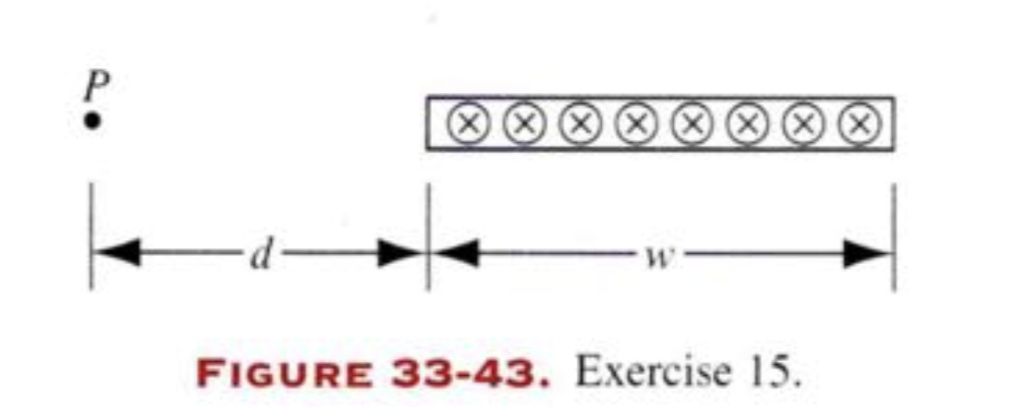
\includegraphics[scale=0.6]{33-43.png}
\end{center}
\end{problem}

\begin{solution}
\vfill
\end{solution}
\newpage


\end{document}
